\documentclass[palatino,nosec]{Docencia}


\title{Examen modelo con solución (4ºA)}

\author{Departamento de Matemáticas}
\date{17/18}


% Paquetes adicionales

\usepackage[author={Víctor de Juan, 2017}]{pdfcomment}

\usepackage{pgf,tikz}
\usetikzlibrary{arrows}


\definecolor{qqttcc}{rgb}{0,0.2,0.8}
\definecolor{qqqqff}{rgb}{0,0,1}
\definecolor{cccccc}{rgb}{0.8,0.8,0.8}


\makeatletter
\newcommand{\annotate}[2][]{%
\pdfstringdef\x@title{#1}%
\edef\r{\string\r}%
\pdfstringdef\x@contents{#2}%
\pdfannot
width 2\baselineskip
height 2\baselineskip
depth 0pt
{
/Subtype /Text
/T (\x@title)
/Contents (\x@contents)
}%
}
\makeatother



\usepackage{eso-pic}
\newcommand\BackgroundPic{%
\put(0,0){%
\parbox[b][\paperheight]{\paperwidth}{%
\vfill
\centering

\includegraphics[width=\paperwidth,height=\paperheight,%
keepaspectratio]{../../../BWLogo.jpeg}%
\vfill
}}}





\begin{abstract}
Examen modelo de ecuaciones con el temario visto en 4ºA. 

\nota{Estos ejemplos no están exentos de erratas. En caso de descubrir alguna, por favor, comunicarlas.}
\end{abstract}

% --------------------
\newcommand{\cimplies}{\text{\hl{$\implies$}}}

\begin{document}
\pagestyle{plain}
\maketitle

\AddToShipoutPicture{\BackgroundPic}

\begin{problem} (1.5 puntos)

Resuelve las siguientes ecuaciones:

\[
	\frac{2x^2+4x+6}{x-1} ≤ x
\]

\solution

\[
	\frac{2x^2+4x+6}{x-1} ≤ x \dimplies \frac{2x^2+4x+6}{x-1}-x≤ 0 \dimplies \frac{2x^2+4x+6-x^2+x}{x-1} ≤ 0 \]
	\[\dimplies \frac{x^2+5x+6}{x-1} ≤ 0 \dimplies \frac{(x+2)(x+3)}{x-1} ≤ 0
\]


\[
\begin{array}{ccccc} 
&(-\infty,-3)&(-3,-2)&(-2,1)&(1,\infty)\\                          
(x-1)&-&-&-&+\\         
(x+2)&-&-&+&+\\         
(x+3)&-&+&+&+\\         
\frac{(x+2)(x+3)}{x-1} 
	 &-&+&-&+
\end{array}     
\]

Solución: $(-∞,-3] ∪ (1,2]$.

\obs El 1 está abierto porque anula el denominador.

\end{problem}

\begin{problem}(1.5 puntos)
Resuelve la siguiente inecuación:

\[
\left\{
\begin{array}{c}
	2x-y+7≥0\\
	x≤7
\end{array}
\right\}
\]

\solution

La solución es donde coinciden los 2 sombreados y por lo tanto es más opaca.

\begin{center}
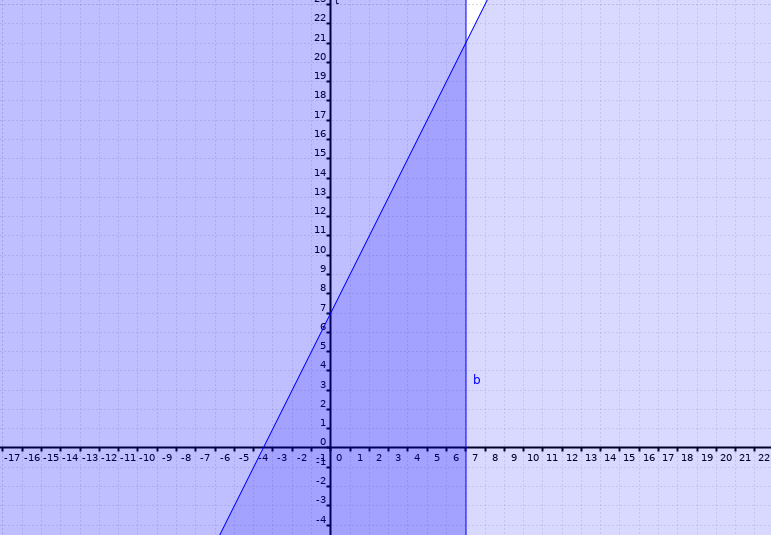
\includegraphics[scale=0.3]{solu}
\end{center}

\end{problem}

\begin{problem} (2 puntos)
En una tienda de comercio justo hay dos tipos de marcas de té:
una de Chad y otra de Níger. En el que procede de Chad, cada paquete
cuesta 0,5 euros, y el de Níger, 1,5 euro. Averigua el número de paquetes
de cada tipo que puedo adquirir si llevo 6 euros en el bolsillo y quiero
comprar el triple de paquetes del elaborado en Chad que del procedente
de Níger.

\solution

$x:$ paquetes de Chad.

$y:$ paquetes de Níger.

Como tiene que haber el triple de Chad que de Níger, $3y=x$ (si tengo uno de Níger, necesito 3 de Chad).

Planteamos la inecuación:

\[
0.5·x + 1.5·\left(\rfrac{x}{3}\right) ≤ 6 \dimplies 0.5x+0.5x ≤ 6 \dimplies x≤6
\]

Solución: como máximo puedes comprar 6 de Chad y 2 de Níger.

\end{problem}

\begin{problem} Calcula:

\spart $sen(-240)$
\spart $cotg(-4π)$

\solution

\ppart $sen(-240) = -sen(240) = +sen(240-180) = sen(60) = \rfrac{\sqrt{3}}{2}$
\ppart $cotg(-4π) = cotg(-4π + 4π) = cotg(0) = \frac{cos(0)}{sen(0)} = \frac{1}{0}, \nexists cotg(0)$. 
\end{problem}


\begin{problem} Sabiendo que y que α = 101,54º ; $cos(α) = \rfrac{-1}{5}$ , halla las
demás razones trigonométricas. Deja los resultados en forma de fracción.
(Cuidado con el signo de las razones trigonométricas)

\solution

Utilizando $cos^2(α) + sen^2(α) = 1$:

\[
sen(α) = \sqrt{1-\left(\rfrac{-1}{5}\right)^2} = \sqrt{\frac{24}{25}} = +\frac{2\sqrt{6}}{5}
\]

Elegiré la raíz positiva porque $α$ está en el segundo cuadrante.



Utilizando $tg(α) = \frac{sen(α)}{cos(α)}$
\[
tg(α) = \frac{sen(α)}{cos(α)} = \frac{\rfrac{2\sqrt{6}}{5}}{\rfrac{-1}{5}} = -2\sqrt{6}
\]


Utilizando $sec(α) = \frac{1}{cos(α)}$
\[
	sec(α) = \frac{1}{cos(α)} = \frac{1}{\rfrac{-1}{5}} = -5
\]

Utilizando $cosec(α) = \frac{1}{sen(α)}$
\[
	cosec(α) = \frac{1}{sen(α)} = \frac{1}{+\frac{2\sqrt{6}}{5}} = \frac{5\sqrt{6}}{12}
\]

Utilizando $cotg(α) = \frac{1}{tg(α)}$
\[
	cotg(α) = \frac{1}{tg(α)} = \frac{1}{-2\sqrt{6}} =  \frac{-\sqrt{6}}{12}
\]
\end{problem}

\begin{problem}
Calcula el perímetro de la figura. Para ello resuelve los tríangulos.

\solution


Resolviendo los ángulos de cada triángulo, obtenemos: $\hat{A} = 60, \hat{B} = 30, \hat{C} = 90$.


Como el ángulo $C$ es un ángulo recto, por lo que podemos utilizar:

\[sen(\hat{B}) = \frac{3cm}{AB} \implies AB = \frac{3}{sen(\hat{B})} = \frac{3}{sen(\hat{30})} = \frac{3}{\rfrac{1}{2}} = 6cm\]

\[cos(\hat{B}) = \frac{BC}{6} \implies BC = 6·{cos(\hat{B})} = 6·{cos(\hat{30})} = \frac{6·\sqrt{3}}{2}}cm \]


El perímetro de la figura es:

\[
	P = 3cm+6cm + \frac{6·\sqrt{3}}{2}}cm = \frac{18+6·\sqrt{3}}{2}}cm
\]

Y como no tengo calculadora, lo dejo así.

\end{problem}

\begin{problem}

Resuelve la siguiente ecuación trigonométrica: $cotg(x) = \sqrt{3}$

\solution

Como $cotg(x)>0$, entonces $tg(x)$ también será positiva. Por lo tanto tendremos soluciones tanto en el primer como en el tercer cuadrante.

\[
cotg(x) = \sqrt{3} \implies tg(x) = \frac{1}{\sqrt{3}}= \frac{\sqrt{3}}{\sqrt{3}\sqrt{3}}= \frac{\sqrt{3}}{3}
\]

Sabemos que $tg(30) = \frac{\sqrt{3}}{3}$, por lo que tenemos que trasladar 30 al primer y tercer cuadrante.

\[
	I \to x_1 = 30 + 360k, ∀k\inℤ
\]

\[
	III \to 30+180 = 210 \to x_2 = 210 + 360k, \;\;∀k\inℤ
\]


\obs Tabmién sería válida la solución $x=30+180k, \;\;∀k∈ℤ$

\end{problem}

\end{document}
